\documentclass[]{elsarticle} %review=doublespace preprint=single 5p=2 column
%%% Begin My package additions %%%%%%%%%%%%%%%%%%%
\usepackage[hyphens]{url}



\usepackage{lineno} % add
\providecommand{\tightlist}{%
  \setlength{\itemsep}{0pt}\setlength{\parskip}{0pt}}

\usepackage{graphicx}
\usepackage{booktabs} % book-quality tables
%%%%%%%%%%%%%%%% end my additions to header

\usepackage[T1]{fontenc}
\usepackage{lmodern}
\usepackage{amssymb,amsmath}
\usepackage{ifxetex,ifluatex}
\usepackage{fixltx2e} % provides \textsubscript
% use upquote if available, for straight quotes in verbatim environments
\IfFileExists{upquote.sty}{\usepackage{upquote}}{}
\ifnum 0\ifxetex 1\fi\ifluatex 1\fi=0 % if pdftex
  \usepackage[utf8]{inputenc}
\else % if luatex or xelatex
  \usepackage{fontspec}
  \ifxetex
    \usepackage{xltxtra,xunicode}
  \fi
  \defaultfontfeatures{Mapping=tex-text,Scale=MatchLowercase}
  \newcommand{\euro}{€}
\fi
% use microtype if available
\IfFileExists{microtype.sty}{\usepackage{microtype}}{}
\bibliographystyle{elsarticle-harv}
\usepackage{longtable}
\ifxetex
  \usepackage[setpagesize=false, % page size defined by xetex
              unicode=false, % unicode breaks when used with xetex
              xetex]{hyperref}
\else
  \usepackage[unicode=true]{hyperref}
\fi
\hypersetup{breaklinks=true,
            bookmarks=true,
            pdfauthor={},
            pdftitle={Building Footprint Identification with Airborne LiDAR: A Final Project for FOR 796},
            colorlinks=false,
            urlcolor=blue,
            linkcolor=magenta,
            pdfborder={0 0 0}}
\urlstyle{same}  % don't use monospace font for urls

\setcounter{secnumdepth}{5}
% Pandoc toggle for numbering sections (defaults to be off)

% Pandoc citation processing
\newlength{\cslhangindent}
\setlength{\cslhangindent}{1.5em}
\newlength{\csllabelwidth}
\setlength{\csllabelwidth}{3em}
% for Pandoc 2.8 to 2.10.1
\newenvironment{cslreferences}%
  {}%
  {\par}
% For Pandoc 2.11+
\newenvironment{CSLReferences}[2] % #1 hanging-ident, #2 entry spacing
 {% don't indent paragraphs
  \setlength{\parindent}{0pt}
  % turn on hanging indent if param 1 is 1
  \ifodd #1 \everypar{\setlength{\hangindent}{\cslhangindent}}\ignorespaces\fi
  % set entry spacing
  \ifnum #2 > 0
  \setlength{\parskip}{#2\baselineskip}
  \fi
 }%
 {}
\usepackage{calc}
\newcommand{\CSLBlock}[1]{#1\hfill\break}
\newcommand{\CSLLeftMargin}[1]{\parbox[t]{\csllabelwidth}{#1}}
\newcommand{\CSLRightInline}[1]{\parbox[t]{\linewidth - \csllabelwidth}{#1}\break}
\newcommand{\CSLIndent}[1]{\hspace{\cslhangindent}#1}

% Pandoc header
\usepackage{float}
\usepackage{booktabs}
\usepackage{longtable}
\usepackage{array}
\usepackage{multirow}
\usepackage{wrapfig}
\usepackage{float}
\usepackage{colortbl}
\usepackage{pdflscape}
\usepackage{tabu}
\usepackage{threeparttable}
\usepackage{threeparttablex}
\usepackage[normalem]{ulem}
\usepackage{makecell}
\usepackage{xcolor}



\begin{document}
\begin{frontmatter}

  \title{Building Footprint Identification with Airborne LiDAR: A Final Project for FOR 796}
    \author[]{Lucas K Johnson}
  
      
  \begin{abstract}
  Airborne LiDAR has emerged as a uniquely valuable and information-rich source
  of remote sensing (RS) data for high-resolution forest assessment and mapping.
  However, LiDAR data is limited in its ability to distinguish man-made
  structures from natural ones, necessitating the addition of external forest
  masks in LiDAR-based forest mapping projects.
  These external masks are often either too inaccurate or too expensive,
  leaving room for an efficient middle way.
  In this report I aimed to produce cost-efficient models that can identify
  buildings in 30m pixels.
  I fit a simple logistic regression model and two machine-learning
  models with a set of 39 LiDAR-derived predictors and open source building
  footprint data.
  Results indicated that both random forests and stochastic gradient boosting
  machines can predict the presence of buildings with a high degree of accuracy
  (AUC = 0.96) given the input data used in this report.
  With further assessment and tuning, these models can likely be used to
  efficiently produce accurate forest masks anywhere high-quality airbone LiDAR
  data has been acquired.

  \,
  \end{abstract}
  
 \end{frontmatter}

\hypertarget{introduction}{%
\section{Introduction}\label{introduction}}

Forest mapping and monitoring is becoming increasingly important as
federal, state, and global agencies look towards natural solutions
to mitigate a warming climate and the myriad resulting challenges.
Field sampling~programs,
like the United States Department of Agriculture's Forest Inventory and Analysis
program (FIA) (Gray et al. 2012),
provide unbiased estimates of forest structure over large areas,
but lack the fine spatial resolution to understand and manage forests at
relevant scales.
Thus, high-resolution forest mapping is needed to inform decision-makers where
forest resources should be managed or preserved.

Airborne LiDAR has been established as the most valuable remote sensing data for
the purposes of forest structure mapping (Huang et al. 2019; Hurtt et al. 2019; Chen and McRoberts 2016).
However, due to the nature of this data and its near-singular ability to
characterize three-dimensional height-profiles,
LiDAR cannot inherently distinguish between man-made structures and woody
vegetation.
To address this challenge, auxiliary landcover or forest canopy masks
are often applied to LiDAR-modeled surfaces in attempt remove erroneous
predictions in buildings from those in forested areas (Huang et al. 2019).
However, it is well documented that landcover maps are not 100\% accurate, and
significant quantities of forest can be contained in non-forested classes
(Johnson et al. 2014; Perry et al. 2008; Meneguzzo, Liknes, and Nelson 2012).
Additionally, high-resolution tree-canopy delineation surfaces are expensive
to produce often relying on expert interpretation and iterative tuning (J. P. M. O'Neil-Dunne et al. 2013; J. O'Neil-Dunne, MacFaden, and Royar 2014).

In this report I attempt to find a middle way by producing models at reduced
cost that can predict the presence of buildings in a mixed-use landscape with a high-degree of accuracy at a 30m resolution.
To do this I train a simple logistic model,
a random forest model, and a stochastic gradient boosting machine to classify
the presence (1) or absence (0) of any buildings in a given map pixel.
Building indicator response data was derived from an open-source building
footprint dataset developed by Microsoft (Microsoft 2018; Team 2018).
The predictor data used to train these models are LiDAR-derived grid metrics, commonly used in models of forest-structure, aiding in the reduction of cost.
If these models prove to be successful classifiers of building presence,
the same predictors will afford future forest-structure modelers double the
benefit.

\hypertarget{methods}{%
\section{Methods}\label{methods}}

\hypertarget{building-and-lidar-data}{%
\subsection{Building and LiDAR Data}\label{building-and-lidar-data}}

Rasterized building footprint data served as the response data in this study
(Pourpeikari Heris et al. 2020; Heris et al. 2020; Team 2018; Microsoft 2018).
The raw raster contains counts of the number of buildings intersecting each
pixel.
This data was converted to a Boolean raster where 1s represent the presence of
any buildings, and 0s represent a complete lack of buildings.
This data was chosen for its availability across the entire country, its high
accuracy (\textgreater{} 99\% positive predictive value), and its 30m resolution
(Heris et al. 2020).

The raw LiDAR data originates from a single acquisition covering the city
of Buffalo and larger portions of Erie, Genesee, and Livingston counties in
western New York (New York Office of Information Technology Services 2019).
This particular data was selected due to its known ability to characterize
three dimensional height-profiles at high-resolution, and the range of
landcover conditions (urban, forest, cropland).
The data was made available by the New York State GIS Program Office.
The raw LiDAR data was height-normalized and converted into a set of 39
predictors (Table \ref{tab:predictors}) chosen for their prevalence in models
of forest structure (Hawbaker et al. 2010; Huang et al. 2019; Pflugmacher et al. 2014).

The LiDAR predictors, in raster stack form, were overlaid with the Boolean
building raster to create stack of data where each pixel contained a set of 39
predictors and one building indicator response variable.
A stratified random sample was conducted on the raster stack, with the building
indicator providing the levels of stratification.
3,500 pixels were selected from each stratum resulting in 7,000 observations for model training and testing.
This final dataset was converted to a 7000x40 (rows, columns) data frame.
The lidR (Roussel and Auty 2020; Jean-Romain et al. 2020) and raster (Hijmans 2021) packages were used for
height-normalization and dataset generation.
Additionally, the first seven principle components were derived from the final dataset to produce an alternative dataset without multicollinearity predictor
dataset (R Core Team 2021).
This alternative dataset accounted for \(\ge\) 95\% of the information in the raw predictors and existed as a 7000x7 data frame.

\begin{table}

\caption{\label{tab:predictors}Definitions of predictors used for model fitting.}
\centering
\begin{tabular}[t]{>{\raggedright\arraybackslash}p{10em}>{\raggedright\arraybackslash}p{22em}}
\toprule
\multicolumn{1}{c}{Predictor} & \multicolumn{1}{c}{Definition}\\
\midrule
H0, H10, ... H100, H95, H99 & Decile heights of returns, in meters, as well as 95th and 99th percentile return heights.\\
\addlinespace
D10, D20... D90 & Density of returns above a certain height, as a proportion. After return height is divided into 10 equal bins ranging from 0 to the maximum height of returns, this value reflects the proportion of returns at or above each breakpoint.\\
\addlinespace
ZMEAN, ZMEAN\_C & Mean height of all returns (ZMEAN) and all returns above 2.5m (ZMEAN\_C)\\
\addlinespace
Z\_KURT, Z\_SKEW & Kurtosis and skewness of height of all returns\\
\addlinespace
QUAD\_MEAN, QUAD\_MEAN\_C & Quadratic mean height of all returns (QUAD\_MEAN) and all returns above 2.5m (QUAD\_MEAN\_C)\\
\addlinespace
CV, CV\_C & Coefficient of variation for heights of all returns (CV) and all returns above 2.5m (CV\_C)\\
\addlinespace
L2, L3, L4, L\_CV, L\_SKEW, L\_KURT & L-moments and their ratios as defined by Hosking (1990), calculated for heights of all returns\\
\addlinespace
CANCOV & Ratio of returns above 2.5m to all returns (Pflugmacher et al. 2012)\\
\addlinespace
HVOL & CANCOV * ZMEAN (Pflugmacher et al. 2012)\\
\addlinespace
RPC1 & Ratio of first returns to all returns (Pflugmacher et al. 2012)\\
\bottomrule
\end{tabular}
\end{table}

\hypertarget{models}{%
\subsection{Models}\label{models}}

Three candidate classification models were fit to a random 70\%
(calibration data; n =
3500
)
of the observations, with the remaining 30\% reserved for model performance
assessment (holdout data; n =
1500
).
The first candidate model was a simple logistic regression model (R Core Team 2021),
and was trained on the principle components variant of the calibration data.
The second candidate model was a random forest (RF herafter) trained with
the ranger R package (Wright and Ziegler 2017).
The third candidate model was a stochastic gradient boosting machine
(LGB hereafter) trained with the LightGBM R package (Ke et al. 2021).
The hyperparemeters for both the RF and LGB models were selected using a
standard grid search where each combination of hyperparameters were compared
against eachother using the cross-entropy loss function
(CEL; Equation \eqref{eq:cel})
computed from a random five-fold cross-validation with the calibration dataset.
CEL is computed as follows:

\begin{equation}
\operatorname{CEL} = \sum_{i=1}^{n}{-\log{(\hat{y_{i}})}} \label{eq:cel}
\end{equation}

Where \(n\) is the number of observations in the fold, and \(\hat{y_i}\) is
the predicted probability of the true class.

Postitive prediction thresholds for all models were chosen using the optimal
ROC coordinates for the fully tuned models fit to the calibration data.
Each of the models were assessed against the holdout dataset and compared to one
another using overall accuracy, specificity, sensitivity, and AUC.
Additionally ROC curves were plotted for each model's results on the holdout
set.
The caret and pROC R packages were used to compute these accuracy metrics
(Kuhn 2021; Robin et al. 2011).

\hypertarget{results}{%
\section{Results}\label{results}}

The RF and LGB models were significantly better than the Logistic model
across all accuracy metrics (Table \ref{tab:metrics}).
While the RF and LGB models shared the same AUC and Overall Accuracy results,
the RF model was sligthly more specific while the LGB model was slightly more sensitive.
However, all three candidate models performed quite well with
all AUC values \(\geq\) 0.87, and all overall accuracies \(\geq\) 0.79.
The ROC curves plotted in Figure \ref{fig:roc} display similar patterns.

\begin{table}

\caption{\label{tab:metrics}Model accuracy metrics computed against holdout partition (n = 1500).}
\centering
\fontsize{12}{14}\selectfont
\begin{tabular}[t]{lrrrr}
\toprule
\multicolumn{1}{c}{Model} & \multicolumn{1}{c}{AUC} & \multicolumn{1}{c}{Overall Accuracy} & \multicolumn{1}{c}{Sensitivity} & \multicolumn{1}{c}{Specificity}\\
\midrule
Logistic & 0.87 & 0.79 & 0.83 & 0.75\\
\addlinespace
RF & 0.96 & 0.90 & 0.92 & 0.89\\
\addlinespace
LGB & 0.96 & 0.90 & 0.90 & 0.90\\
\bottomrule
\end{tabular}
\end{table}

\begin{figure}
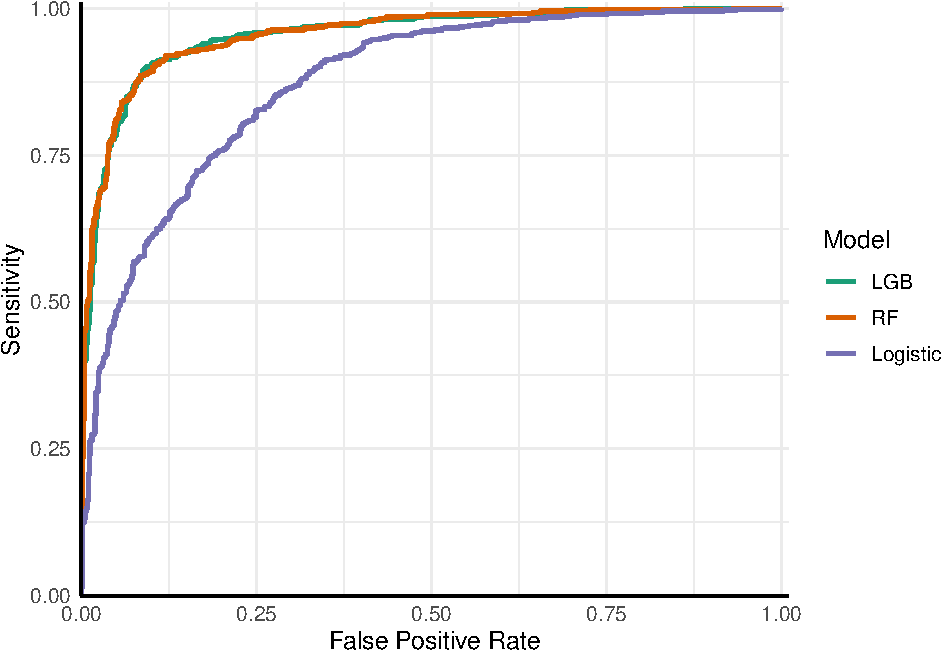
\includegraphics[width=1\linewidth]{report_files/figure-latex/roc-1} \caption{ROC curves for three models tested against the holdout partition (n = 1500).}\label{fig:roc}
\end{figure}

\hypertarget{discussion}{%
\section{Discussion}\label{discussion}}

It is unsurprising that the two machine learning models (RF and LGB)
outperformed the simple Logistic regression model given the constraints
on multicollinearity required for Logistic regression.
In particular, the Logistic model might have been improved by including more
principle components, as in this case we limited the input data to the first
seven principle components which accounted for 95\% of the information in the
raw predictors.
This may have been an unfair disadvantage as the RF and LGB models were given
the opportunity to leverage 100\% of the information in the predictor space.

There are a few ways I could further improve the models described in this
report.
First, more extensive grid searches could have been performed to find better
hyperparameters.
There is a trade-off here between the combination of time
and performance gains, with eventually diminishing returns on the time invested.
The relatively limited tuning performed in this report produced models that were
good enough for my purposes.
Additionally, I might be able to produce an even better model by using
stacked ensembles, which often serve to reduce predictive error, especially
when the error from component models is dominated by variance (Dormann et al. 2018).
Noisy data, which we can assume categorizes our LiDAR and building data, often
yields models with variance dominated error (Dormann et al. 2018).
One potential source of error in our models is the temporal match between
predictor and response data used to fit the models.
The building data, though published in 2018, has no associated
time-of-acquisition requiring us to hope that the building classifications
describe conditions close to those represented in the 2019 LiDAR acquisition
(Heris et al. 2020).

Since the predictors used to train these models are primarily used for
predicting forest structure, these models provide a relatively simple option
to mask man-made structures from LiDAR-derived maps of forest structure like
aboveground biomass or canopy height.
Further investigation is required to assess the transferrability of these models
trained in one region with one LiDAR acquisition to others.
If separate models are required for each distinct LiDAR acquisition or region,
the relative benefit of the models developed in this report would only be
slightly diminsihed, as these models would still serve as a reference point for
other applications.
Finally, a true accuracy assessment, using time-relevant reference data of
higher quality than the building data used herein should be conducted to assess
the suitability of these models in real-world applications (Stehman and Foody 2019).

\newpage{}

\hypertarget{references}{%
\section*{References}\label{references}}
\addcontentsline{toc}{section}{References}

\hypertarget{refs}{}
\begin{CSLReferences}{1}{0}
\leavevmode\vadjust pre{\hypertarget{ref-rmd_man}{}}%
Allaire, JJ, Yihui Xie, Jonathan McPherson, Javier Luraschi, Kevin Ushey, Aron Atkins, Hadley Wickham, Joe Cheng, Winston Chang, and Richard Iannone. 2021. \emph{Rmarkdown: Dynamic Documents for r}. \url{https://github.com/rstudio/rmarkdown}.

\leavevmode\vadjust pre{\hypertarget{ref-Chen2016}{}}%
Chen, Qi, and Ronald McRoberts. 2016. {``Statewide Mapping and Estimation of Vegetation Aboveground Biomass Using Airborne Lidar.''} In \emph{2016 {IEEE} International Geoscience and Remote Sensing Symposium ({IGARSS})}. {IEEE}. \url{https://doi.org/10.1109/igarss.2016.7730157}.

\leavevmode\vadjust pre{\hypertarget{ref-Dormann2018}{}}%
Dormann, Carsten F., Justin M. Calabrese, Gurutzeta Guillera-Arroita, Eleni Matechou, Volker Bahn, Kamil Bartoń, Colin M. Beale, et al. 2018. {``Model Averaging in Ecology: A Review of Bayesian, Information-Theoretic, and Tactical Approaches for Predictive Inference.''} \emph{Ecological Monographs} 88 (4): 485--504. \url{https://doi.org/10.1002/ecm.1309}.

\leavevmode\vadjust pre{\hypertarget{ref-Gray2012}{}}%
Gray, Andrew N, Thomas J Brandeis, John D Shaw, William H McWilliams, and Patrick Miles. 2012. {``Forest Inventory and Analysis Database of the United States of America (FIA).''} \emph{Biodiversity and Ecology} 4: 225--31. \url{https://doi.org/10.7809/b-e.00079}.

\leavevmode\vadjust pre{\hypertarget{ref-Hawbaker2010}{}}%
Hawbaker, Todd J., Terje Gobakken, Adrian Lesak, Eric Trømborg, Kirk Contrucci, and Volker Radeloff. 2010. {``{Light Detection and Ranging-Based Measures of Mixed Hardwood Forest Structure}.''} \emph{Forest Science} 56 (3): 313--26. \url{https://doi.org/10.1093/forestscience/56.3.313}.

\leavevmode\vadjust pre{\hypertarget{ref-tidyselect}{}}%
Henry, Lionel, and Hadley Wickham. 2021. \emph{Tidyselect: Select from a Set of Strings}. \url{https://CRAN.R-project.org/package=tidyselect}.

\leavevmode\vadjust pre{\hypertarget{ref-Heris2020b}{}}%
Heris, Mehdi P., Nathan Leon Foks, Kenneth J. Bagstad, Austin Troy, and Zachary H. Ancona. 2020. {``A Rasterized Building Footprint Dataset for the United States''} 7 (1). \url{https://doi.org/10.1038/s41597-020-0542-3}.

\leavevmode\vadjust pre{\hypertarget{ref-Raster2021}{}}%
Hijmans, Robert J. 2021. \emph{Raster: Geographic Data Analysis and Modeling}. \url{https://CRAN.R-project.org/package=raster}.

\leavevmode\vadjust pre{\hypertarget{ref-Hosking1990}{}}%
Hosking, J. R. M. 1990. {``L-Moments: Analysis and Estimation of Distributions Using Linear Combinations of Order Statistics.''} \emph{Journal of the Royal Statistical Society. Series B (Methodological)} 52 (1): 105--24. \url{http://www.jstor.org/stable/2345653}.

\leavevmode\vadjust pre{\hypertarget{ref-Huang2019}{}}%
Huang, Wenli, Katelyn Dolan, Anu Swatantran, Kristofer Johnson, Hao Tang, Jarlath O'Neil-Dunne, Ralph Dubayah, and George Hurtt. 2019. {``High-Resolution Mapping of Aboveground Biomass for Forest Carbon Monitoring System in the Tri-State Region of Maryland, Pennsylvania and Delaware, {USA}.''} \emph{Environmental Research Letters} 14 (9): 095002. \url{https://doi.org/10.1088/1748-9326/ab2917}.

\leavevmode\vadjust pre{\hypertarget{ref-Hurtt2019}{}}%
Hurtt, G, M Zhao, R Sahajpal, A Armstrong, R Birdsey, E Campbell, K Dolan, et al. 2019. {``Beyond {MRV}: High-Resolution Forest Carbon Modeling for Climate Mitigation Planning over Maryland, {USA}.''} \emph{Environmental Research Letters} 14 (4): 045013. \url{https://doi.org/10.1088/1748-9326/ab0bbe}.

\leavevmode\vadjust pre{\hypertarget{ref-lidrRSE}{}}%
Jean-Romain, Roussel, David Auty, Nicholas C. Coops, Piotr Tompalski, Tristan R. H. Goodbody, Andrew Sánchez Meador, Jean-François Bourdon, Florian de Boissieu, and Alexis Achim. 2020. {``lidR: An r Package for Analysis of Airborne Laser Scanning (ALS) Data.''} \emph{Remote Sensing of Environment} 251: 112061. \url{https://doi.org/10.1016/j.rse.2020.112061}.

\leavevmode\vadjust pre{\hypertarget{ref-Johnson2014}{}}%
Johnson, Kristofer D, Richard Birdsey, Andrew O Finley, Anu Swantaran, Ralph Dubayah, Craig Wayson, and Rachel Riemann. 2014. {``Integrating Forest Inventory and Analysis Data into a {LIDAR}-Based Carbon Monitoring System.''} \emph{Carbon Balance and Management} 9 (1). \url{https://doi.org/10.1186/1750-0680-9-3}.

\leavevmode\vadjust pre{\hypertarget{ref-Guolin2021}{}}%
Ke, Guolin, Damien Soukhavong, James Lamb, Qi Meng, Thomas Finley, Taifeng Wang, Wei Chen, Weidong Ma, Qiwei Ye, and Tie-Yan Liu. 2021. \emph{Lightgbm: Light Gradient Boosting Machine}. \url{https://CRAN.R-project.org/package=lightgbm}.

\leavevmode\vadjust pre{\hypertarget{ref-caret}{}}%
Kuhn, Max. 2021. \emph{Caret: Classification and Regression Training}. \url{https://CRAN.R-project.org/package=caret}.

\leavevmode\vadjust pre{\hypertarget{ref-Meneguzzo2012}{}}%
Meneguzzo, Dacia M., Greg C. Liknes, and Mark D. Nelson. 2012. {``Mapping Trees Outside Forests Using High-Resolution Aerial Imagery: A Comparison of Pixel- and Object-Based Classification Approaches.''} \emph{Environmental Monitoring and Assessment} 185 (8): 6261--75. \url{https://doi.org/10.1007/s10661-012-3022-1}.

\leavevmode\vadjust pre{\hypertarget{ref-Microsoft}{}}%
Microsoft. 2018. {``{US Building Footprints.}''} Microsoft.

\leavevmode\vadjust pre{\hypertarget{ref-EGL_Lidar}{}}%
New York Office of Information Technology Services. 2019. {``{LIDAR collection (QL2) for Erie, Genesee, and Livingston Counties New York Lidar; Classified Point Cloud}.''}

\leavevmode\vadjust pre{\hypertarget{ref-Jarlath2013}{}}%
O'Neil-Dunne, Jarlath P. M., Sean W. MacFaden, Anna R. Royar, and Keith C. Pelletier. 2013. {``An Object-Based System for LiDAR Data Fusion and Feature Extraction.''} \emph{Geocarto International} 28 (3): 227--42. \url{https://doi.org/10.1080/10106049.2012.689015}.

\leavevmode\vadjust pre{\hypertarget{ref-Jarlath2014}{}}%
O'Neil-Dunne, Jarlath, Sean MacFaden, and Anna Royar. 2014. {``A Versatile, Production-Oriented Approach to High-Resolution Tree-Canopy Mapping in Urban and Suburban Landscapes Using GEOBIA and Data Fusion.''} \emph{Remote Sensing} 6 (12): 12837--65. \url{https://doi.org/10.3390/rs61212837}.

\leavevmode\vadjust pre{\hypertarget{ref-Perry2008}{}}%
Perry, C. H., C. W. Woodall, G. C. Liknes, and M. M. Schoeneberger. 2008. {``Filling the Gap: Improving Estimates of Working Tree Resources in Agricultural Landscapes.''} \emph{Agroforestry Systems} 75 (1): 91--101. \url{https://doi.org/10.1007/s10457-008-9125-6}.

\leavevmode\vadjust pre{\hypertarget{ref-Pflugmacher2014}{}}%
Pflugmacher, Dirk, Warren B. Cohen, Robert E. Kennedy, and Zhiqiang Yang. 2014. {``Using Landsat-Derived Disturbance and Recovery History and Lidar to Map Forest Biomass Dynamics.''} \emph{Remote Sensing of Environment} 151: 124--37. \url{https://doi.org/10.1016/j.rse.2013.05.033}.

\leavevmode\vadjust pre{\hypertarget{ref-Heris2020a}{}}%
Pourpeikari Heris, Mehdi, Nathan Foks, Kenneth J Bagstad, and Austin Troy. 2020. {``A National Dataset of Rasterized Building Footprints for the u.s.''} U.S. Geological Survey. \url{https://doi.org/10.5066/P9J2Y1WG}.

\leavevmode\vadjust pre{\hypertarget{ref-RCore}{}}%
R Core Team. 2021. \emph{R: A Language and Environment for Statistical Computing}. Vienna, Austria: R Foundation for Statistical Computing. \url{https://www.R-project.org/}.

\leavevmode\vadjust pre{\hypertarget{ref-pROC}{}}%
Robin, Xavier, Natacha Turck, Alexandre Hainard, Natalia Tiberti, Frédérique Lisacek, Jean-Charles Sanchez, and Markus Müller. 2011. {``pROC: An Open-Source Package for r and s+ to Analyze and Compare ROC Curves.''} \emph{BMC Bioinformatics} 12: 77.

\leavevmode\vadjust pre{\hypertarget{ref-lidrCRAN}{}}%
Roussel, Jean-Romain, and David Auty. 2020. \emph{Airborne LiDAR Data Manipulation and Visualization for Forestry Applications}. \url{https://cran.r-project.org/package=lidR}.

\leavevmode\vadjust pre{\hypertarget{ref-Stehman2019}{}}%
Stehman, Stephen V., and Giles M. Foody. 2019. {``Key Issues in Rigorous Accuracy Assessment of Land Cover Products''} 231 (September): 111199. \url{https://doi.org/10.1016/j.rse.2019.05.018}.

\leavevmode\vadjust pre{\hypertarget{ref-Bing}{}}%
Team, Bing Maps. 2018. {``{Computer Generated Building Footprints for the United States.}''} Microsoft.

\leavevmode\vadjust pre{\hypertarget{ref-ggplot2}{}}%
Wickham, Hadley. 2016. \emph{Ggplot2: Elegant Graphics for Data Analysis}. Springer-Verlag New York. \url{https://ggplot2.tidyverse.org}.

\leavevmode\vadjust pre{\hypertarget{ref-dplyr}{}}%
Wickham, Hadley, Romain François, Lionel Henry, and Kirill Müller. 2021. \emph{Dplyr: A Grammar of Data Manipulation}. \url{https://CRAN.R-project.org/package=dplyr}.

\leavevmode\vadjust pre{\hypertarget{ref-Wright2017}{}}%
Wright, Marvin N., and Andreas Ziegler. 2017. {``Ranger: A Fast Implementation of Random Forests for High Dimensional Data in c++ and r.''} \emph{Journal of Statistical Software, Articles} 77 (1): 1--17. \url{https://doi.org/10.18637/jss.v077.i01}.

\leavevmode\vadjust pre{\hypertarget{ref-rmd_guide}{}}%
Xie, Yihui, J. J. Allaire, and Garrett Grolemund. 2018. \emph{R Markdown: The Definitive Guide}. Boca Raton, Florida: Chapman; Hall/CRC. \url{https://bookdown.org/yihui/rmarkdown}.

\leavevmode\vadjust pre{\hypertarget{ref-rmd_cook}{}}%
Xie, Yihui, Christophe Dervieux, and Emily Riederer. 2020. \emph{R Markdown Cookbook}. Boca Raton, Florida: Chapman; Hall/CRC. \url{https://bookdown.org/yihui/rmarkdown-cookbook}.

\leavevmode\vadjust pre{\hypertarget{ref-kbl}{}}%
Zhu, Hao. 2021. \emph{kableExtra: Construct Complex Table with 'Kable' and Pipe Syntax}.

\end{CSLReferences}


\end{document}
